\documentclass[tikz,border=0mm]{standalone} % specifies the border  
%\usetikzlibrary{positioning,fit,calc} % used for the efficient working of the positioning system  
%\tikzset{block/.style={draw, thick, text width=3cm, minimum height=1.5cm, align=center},   
%% the align command is used to align the block diagram at the center  
%% the height command adjust the height of the block diagram  
%% here block diagram refers to the whole diagram, not the single block  
%% the thick command here signifies the border of all the blocks used inside the block diagram. You can change it to thin command if you want the thin edge of the blocks  
%line/.style={-latex}   % the lesser the width the greater will be the diagram window  
%} 

\usepackage{tikz}%1
\usetikzlibrary{shapes,arrows}%2
\usetikzlibrary{positioning,arrows.meta,positioning, fit, calc}

\usetikzlibrary{positioning, fit, calc}   
\usepackage{xcolor}  
\tikzset{block/.style={draw, thick, text width=5cm , minimum height=1.cm, align=center},   
	line/.style={-latex}     
}  
\begin{document}  
  
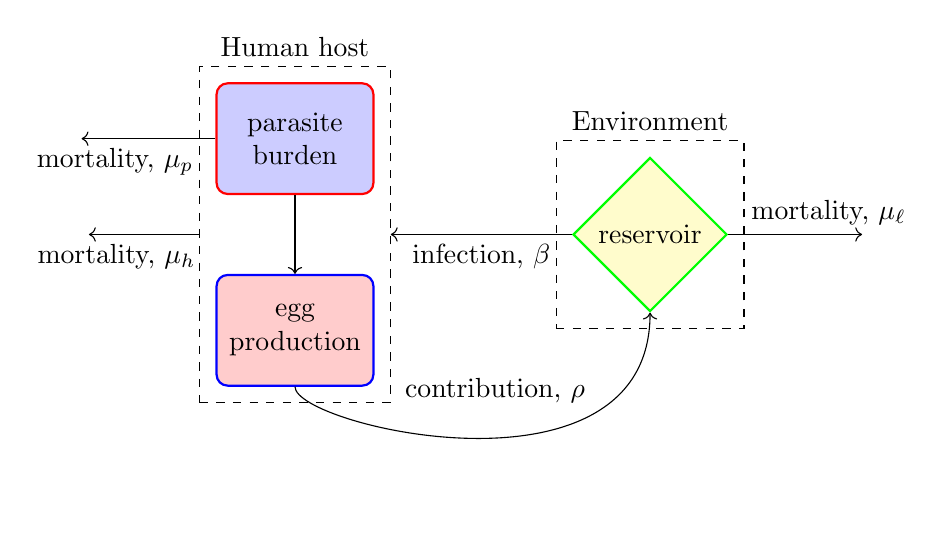
\begin{tikzpicture}[auto]
\tikzstyle{decision} = [diamond, draw=green, thick, fill=yellow!20,
text width=4.5em, text badly centered, inner sep=1pt]
\tikzstyle{block} = [rectangle, draw=red, thick, fill=blue!20,
text width=5em, text centered, rounded corners, minimum height=4em]
\tikzstyle{blockR} = [rectangle, draw=blue, thick, fill=red!20,
text width=5em, text centered, rounded corners, minimum height=4em]
\tikzstyle{line} = [draw, thick, -latex’,shorten >=2pt];
\tikzstyle{cloud} = [draw=red, thick, ellipse,fill=red!20, minimum height=2em];


\node [block] (P) {parasite burden};
\node [blockR,below= of P] (E) {egg production};
\node[draw , dashed , fill=pink, fill opacity=0.0,inner xsep=2mm,inner  
ysep=2mm,fit=(P)(E),label={90:Human host}](H){}; % here label command is used to label the block, which covers block D and E.

\node [decision, right=2.3cm of H] (R) {reservoir};
\node[draw, dashed ,  fill=pink, fill opacity=0.0,inner xsep=2mm,inner  
ysep=2mm,fit=(R),label={90:Environment}](A){}; % he

\node [left=1.7cm  of P](MP){};
\node [right=1.7cm of R](MR){};
\node [left=1.4cm  of H](MH){};

%Lines
\draw[->] (P.south) -- (E.north) node[right] {};

\draw[->] (E.south)  .. controls +(down:5mm) and +(down:25mm) .. (R.south) node [near end] {contribution, $\rho$} ;


%\draw[->] (P.south) -- (E.north) node[right] {};

\draw[->] (P.west) -- (MP.east)  node [near end] {mortality, $\mu_{p}$};

\draw[->] (H.west) -- (MH.east)  node [near end] {mortality, $\mu_{h}$};

\draw[->] (R.east) -- (MR.west)  node [near end] {mortality, $\mu_{\ell}$};

\draw[->] (R.west)  -- (H.east)  node [midway] {infection, $\beta$};

%\draw[->] (E.west)  -- (R.east)  node [midway] {contribution, $\beta$};






%\matrix [column sep=5mm,row sep=7mm]
%{
%	% row 1
%	\node [cloud] (expert) {expert};
%	\node [cloud,right=3cm  of expert] (expert) {expert};
%	 &
%	\node [block] (init) {initialize model}; &
%	\node [cloud] (system) {system}; \\
%	% row 2
%	& \node [block] (identify) {identify candidate model}; & \\
%	% row 3
%	\node [block] (update) {update model}; &
%	\node [block] (evaluate) {evaluate candidate models}; & \\
%	% row 4
%	& \node [decision] (decide) {is best candidate}; & \\
%	% row 5
%	& \node [block] (stop) {stop}; & \\
%};
\tikzstyle{every path}=[line]
%\path (init) -- (identify);
%\path (identify) -- (evaluate);
%\path (evaluate) -- (decide);
%\path (update) |- (identify);
%\path (decide) -| node [near start] {yes} (update);
%\path (decide) -- node [midway] {no} (stop);
%\path [dashed] (expert) -- (init);
%\path [dashed] (system) -- (init);
%\path [dashed] (system) |- (evaluate);
\end{tikzpicture}	












\end{document}  